In addition to the di-photon candidate as described in last section, it is required to have exactly zero leptons (passing the lepton selection defined in previous section) and at least four AK4 jets.
The requirement of zero leptons was added so that there won't be any overlap with the semi-leptonic and fully-leptonic channel of WW while combination.
% Events fall into the FH analysis category if they contain exactly zero leptons, and at least four AK4 jets. 
Additionally, the leading (sub-leading) photon \pt associated with the diphoton candidate is required to have a ratio to the diphoton candidate's 
invariant mass of at least 1/3 (1/4). A selection is not made on b-tagging score as a preselection, in order to use this as an input feature to the DNN in order to allow it to learn how best to use this score for event discrimination.

The Fully-Hadronic $HH\rightarrow WW\gamma\gamma$ channel phase-space has a large overlap with the $HH\rightarrow bb\gamma\gamma$,
and Fully-Hadronic $HH\rightarrow ZZ\gamma\gamma$ processes. Due to the difficulty in differentiating these similar di-Higgs final states, the contributions coming from these two additional channels
are treated as signal. This analysis is optimized for the $WW\gamma\gamma$ final state, in which hadronic W decays including b-jets are very rare. Therefore, events with b-jet candidates should be removed.
For this, a binary DNN was setup, acting as a ``$bb\gamma\gamma$ killer".
This helps remove the large contamination from the $bb\gamma\gamma$ and Fully-Hadronic $ZZ\gamma\gamma$ processes.
For the $bb\gamma\gamma$ killer DNN, a $bb\gamma\gamma$ sample was used as a signal. The list
of backgrounds used for the training includes Fully-Hadronic $WW\gamma\gamma$, diphoton, $\gamma+$jets, QCD, $tt\gamma\gamma$, and $tt\gamma$.

The dominating background for the Fully-Hadronic, channel is QCD and $\gamma+$jets. In order to get the proper modelling of these background, it is computed from the data itself, where one photon candidate is failing the requirement of the photon ID~\cite{Sirunyan:2020sum}.

% The modelling of QCD and $\gamma+$jets has a large underprediction in MC. This comes from the lower region of minimum photon ID MVA, defined as the minimum value of the photon MVA scores 
% between the two photon candidates from the highest $\pt$ diphoton candidate in the event. In order to properly model these processes,
% their shapes are defined using a data-driven technique using the data sideband, defined as the regions 100-115 and 135-180 GeV in the $m_{\gamma\gamma}$ spectrum, 
% where a QCD and $\gamma+$jets dominant region in data, the low photon ID side-band (ID $<$ -0.7), is used to model these processes. 
% This is performed in a similar way as described in \cite{Sirunyan:2020sum}.
% The overall normalization of events from the low photon ID
% side-band region should not be expected, a priori, to be the same as the number of QCD and $\gamma$+jets events in the pre-selection.
% To address this, a simultaneous fit in the minimum and maximum photon ID MVA's, defined as the lower and greater photon ID values between the two photons making up the 
% highest $\pt$ diphoton candidate in each event, is performed. This includes a simultaneous fit to data in the high-ID region (ID$>$-0.7) in the data sidebands, with the addition of 
% $\gamma\gamma+$jets and tt from MC, to extract the QCD $+$ $\gamma+$jets normalization.

Additionally, a fully-connected binary DNN is trained in order to separate Fully-Hadronic WW$\gamma\gamma$ events from all other background events.
For this the list of backgrounds includes diphoton, $\gamma+$jets, QCD, $tt\gamma\gamma$ and $tt\gamma$.
Apart from the signal and background lists, the network architecture and input variables are the same as for the bb$\gamma\gamma$ killer DNN. The input features 
used for training of both DNN's are shown in Fig. \ref{fig:DNNinputvars}. Note that the FH DNNs make the use of additional jet information not available in the SL final state, described in Sec. \ref{sec:SL_Event_Selection}. 

The most important variables for the bb$\gamma\gamma$ killer, according to their Shapley ranking \cite{shapley_values}, are
the sum of b-tagging scores of the two jets with the highest b-tagging scores, $\Delta R (\gamma\gamma) (=\sqrt{\Delta \phi^2 + \Delta \eta^2})$,
leading jet b-tagging score, ratio of leading photon $\pt$ to the diphoton mass, leading jet $\pt$,  vector sum of $\pt$ of the leading four jets,
b-tagging score of sub-leading jet, invariant mass of the system of the four leading $\pt$ jets, and minimum $\Delta R$ separation between
diphoton candidate and the four leading jets.

The most important variables for signal extraction, according to their Shapley ranking, are $\Delta R (\gamma\gamma)$, 
ratio of the leading and sub-leading photon $\pt$'s to the diphoton mass,
leading 2 jet invariant mass, leading 4 jet invariant mass, minimum $\Delta R$ separation between
the diphoton candidate and the four leading jets, and the sum of b-tagging scores among the two jets with the highest
b-tagging scores. Fig.~\ref{fig:FH_DataMC_1} and~\ref{fig:FH_DataMC_2} shows the data/MC comparison plots for the top three ranked variables of the DNN and the DNN score.

After computing the DNN output score for each event, events are placed into categories based on DNN score in order to maximize the sensitivity of the DNN categorization. 
To optimize the expected sensitivity, the expected ratio of signal yield to the square root of background yield in the signal region is computed using MC while varying the number of categories and bins. 
Additionally, a signal region definition of 122 to 128 GeV is used as this is the experimental resolution: A range centered aroudn the expected Higgs mass with a width roughly 1-2 times 
the expected signal width. Four categories are defined, with the corresponding DNN score boundaries: [0.1, 0.893, 0.969, 0.983, 1.0].

In this analysis, events with an HH$\rightarrow$WW$\gamma\gamma$ identifier DNN score less than 0.1 
are removed, and therefore are not used in categorization, nor in any analytic fitting. This is done because this region contains a large portion of background, and a very low portion of signal, and therefore has a negligible impact on the sensitivity of the analysis. Additionally,
this region is not used as a control region to reduce the uncertainty of MC in the signal region.

% Note that as the DNN output score is used to categorize events but is not used as a shape in the extraction of any results, any disagreements 
% between data and simulation could lead to a sub-optimal network, but would not lead to any bias in the 
% final results. 

\begin{figure}[!htbp]
  \centering
  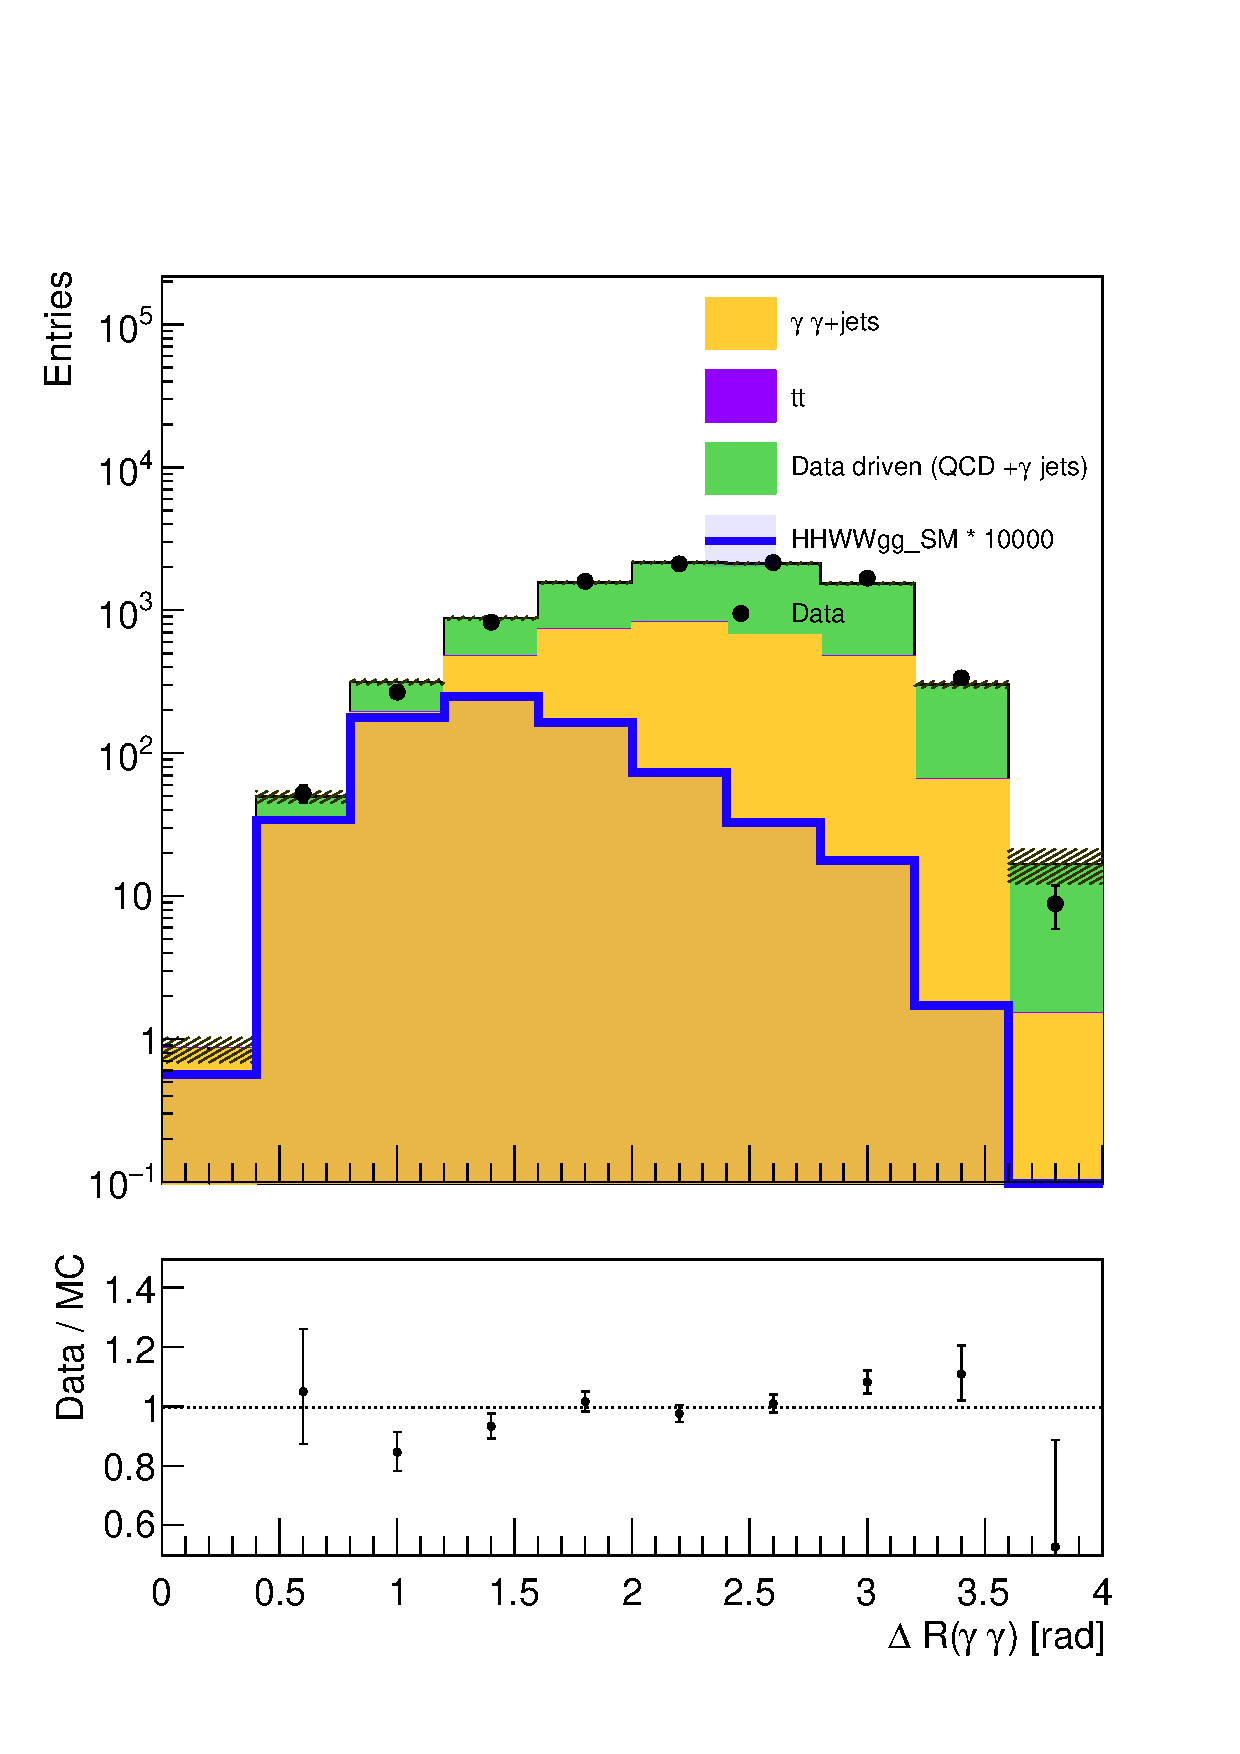
\includegraphics[width=0.45\textwidth]{Images/DataMC/DataMC_New_DR_gg_SB_log.pdf}%
  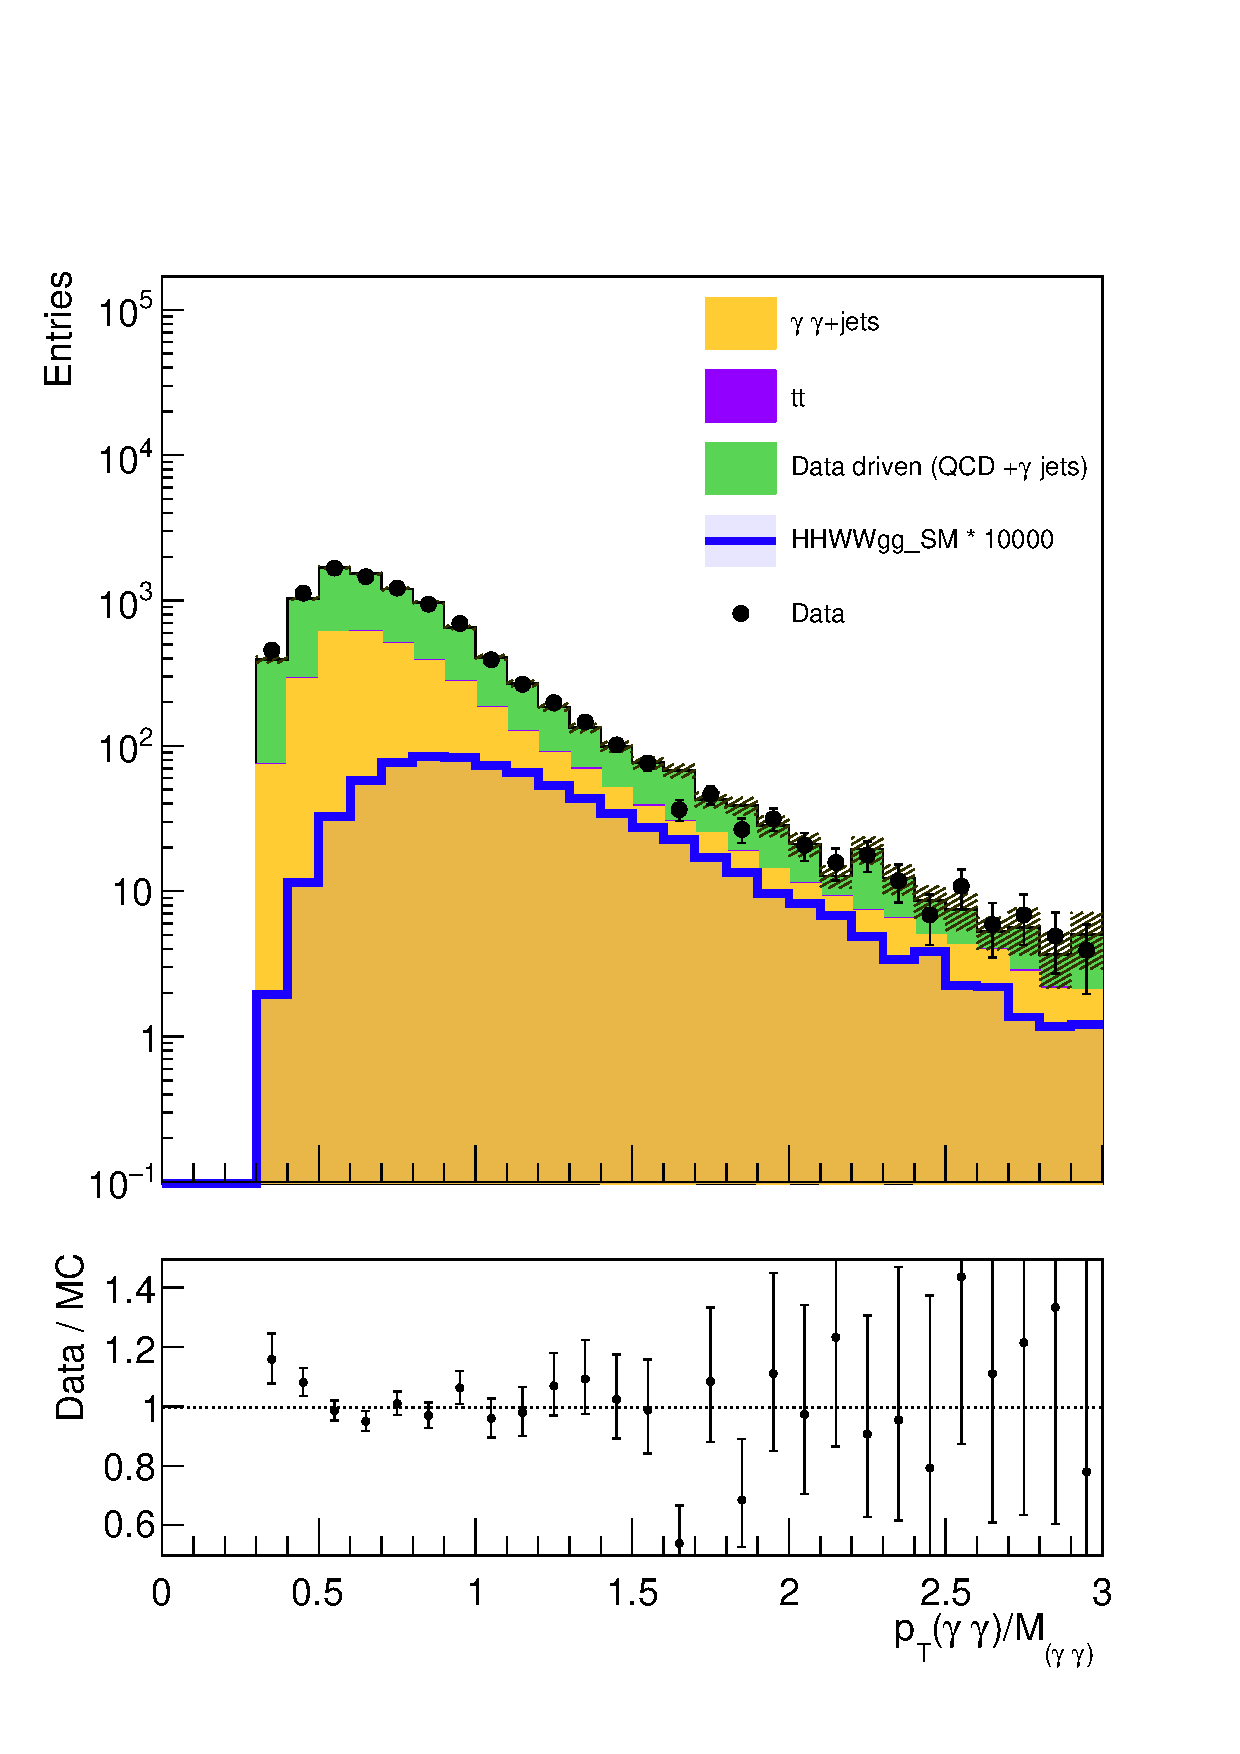
\includegraphics[width=0.45\textwidth]{Images/DataMC/DataMC_Scaled_Leading_Photon_pt_SB_log.pdf}%
  \caption{Data/MC comparison of a fully-hadronic leading DNN input feature (left) and second leading DNN input feature (right).}
\label{fig:FH_DataMC_1}
\end{figure}

\begin{figure}[!htbp]
  \centering
  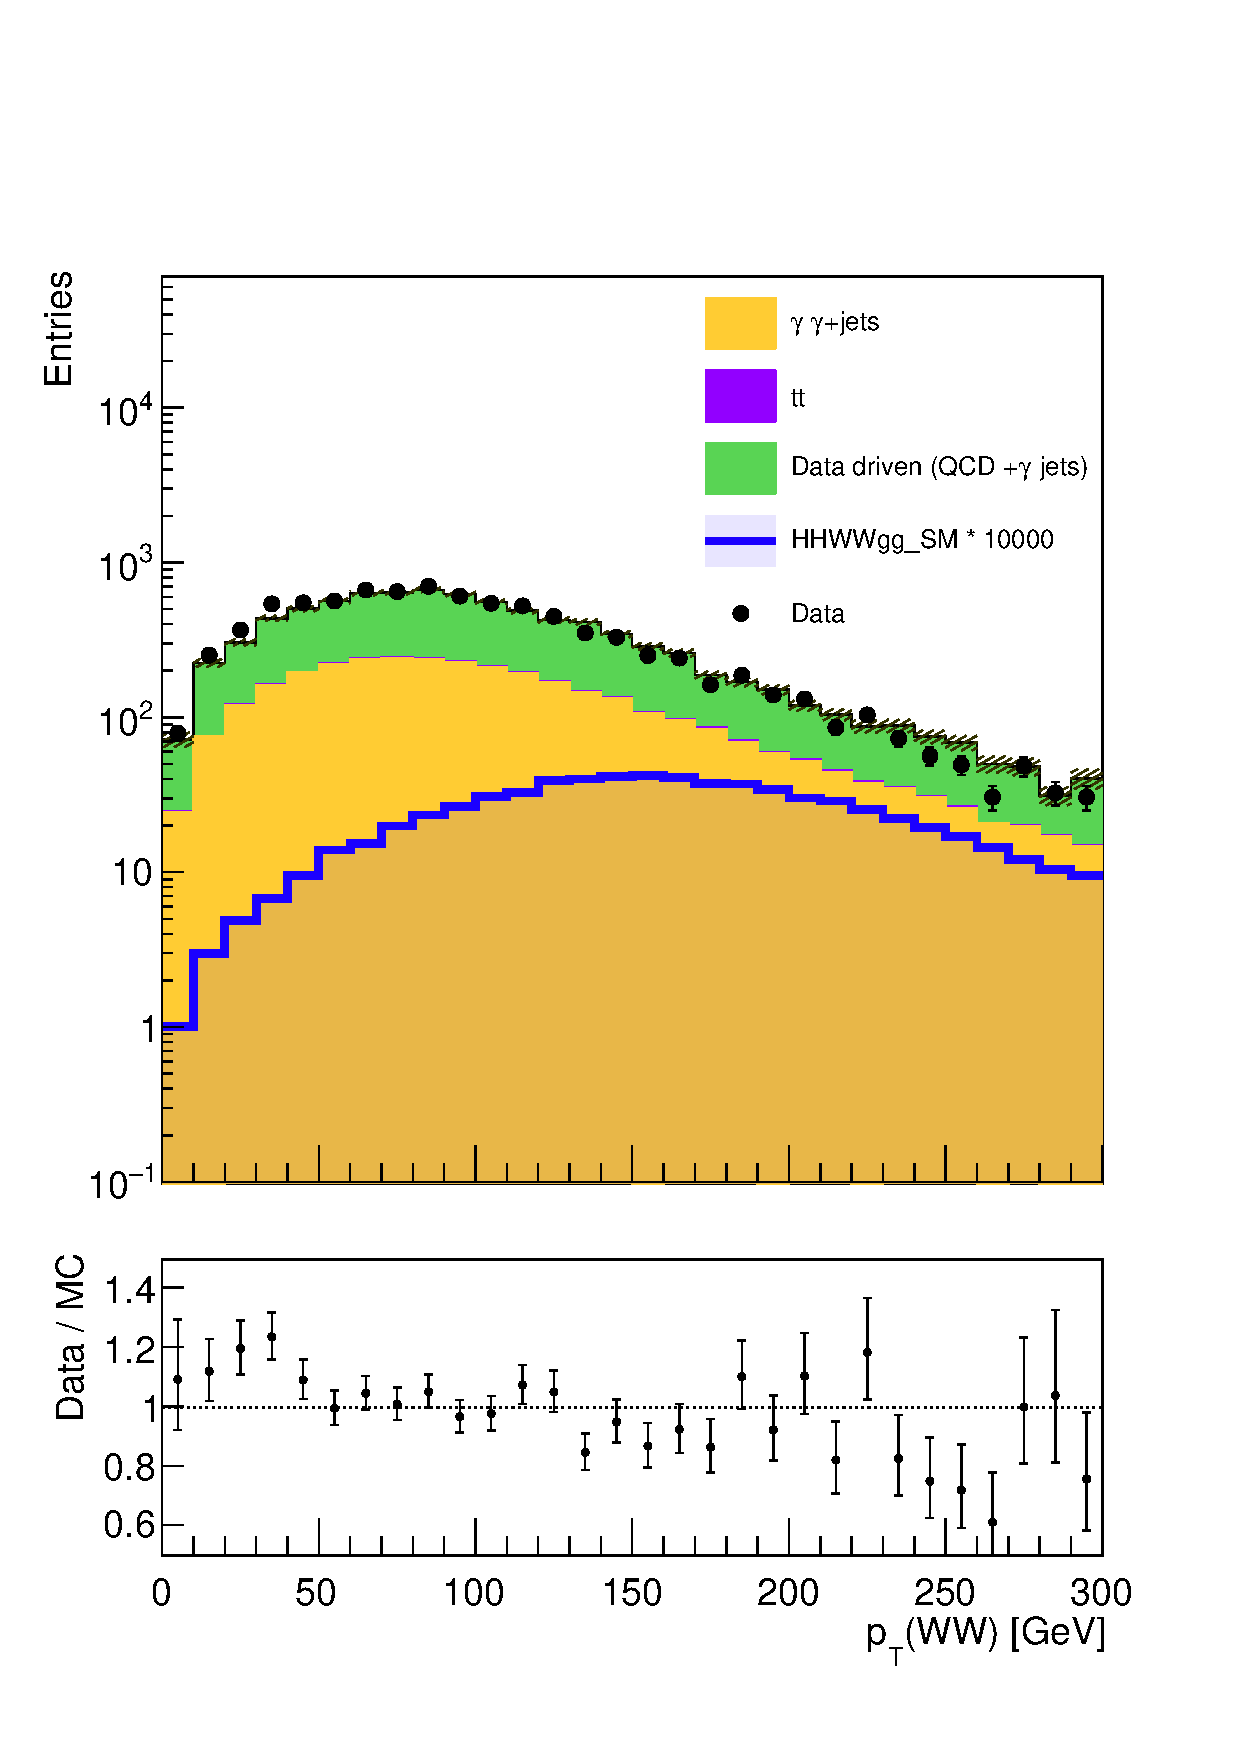
\includegraphics[width=0.45\textwidth]{Images/DataMC/DataMC_New_pTBasedSel_WW_pT_SB_log.pdf}%
  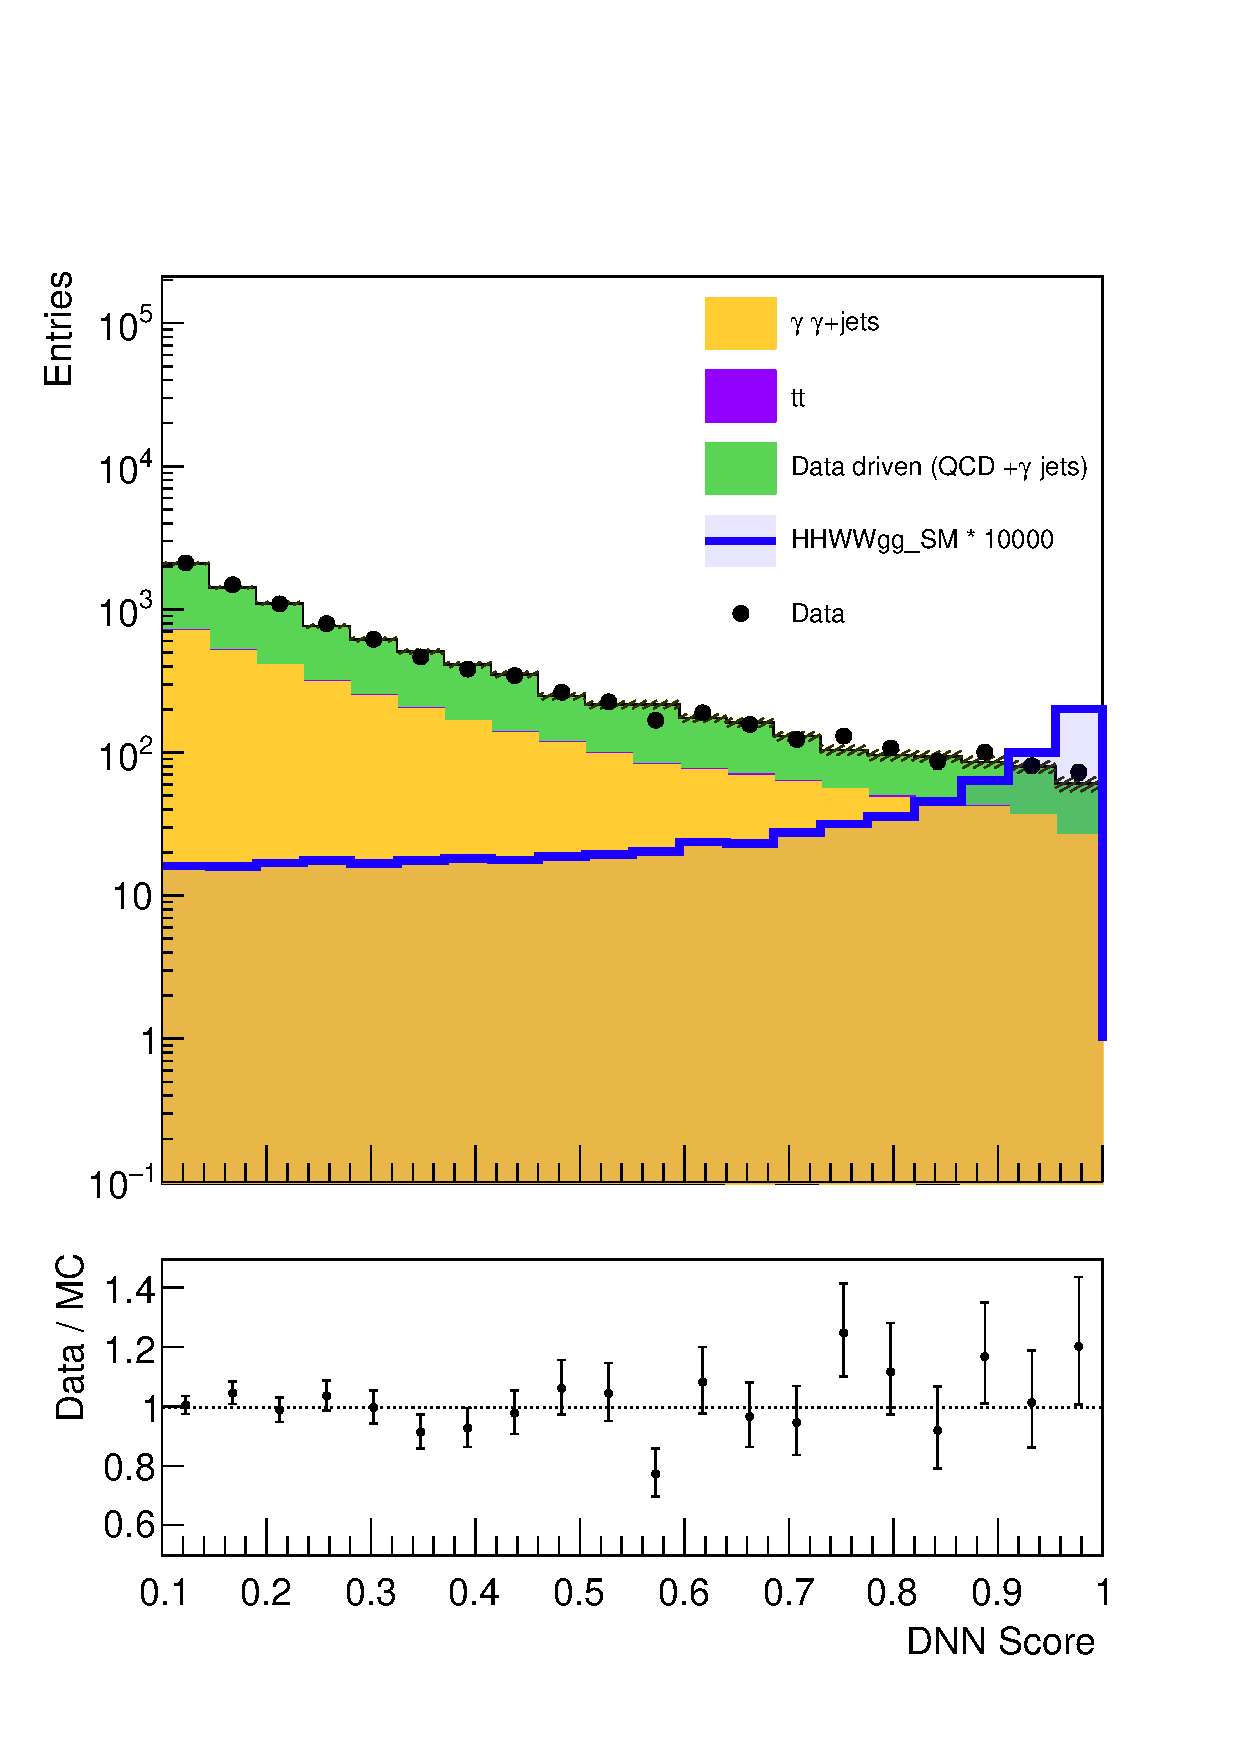
\includegraphics[width=0.45\textwidth]{Images/DataMC/DataMC_evalDNN_WWvsAll_SB_log.pdf}%
  \caption{Data/MC comparison of a fully-hadronic third leading DNN input feature and DNN score.}
\label{fig:FH_DataMC_2}
\end{figure}